%Die Angabe des schlauen Spruchs auf diesem Wege funtioniert nur,
%wenn keine Änderung des Kapitels mittels den in preambel/chapterheads.tex
%vorgeschlagenen Möglichkeiten durchgeführt wurde.
\chapter{Machine Learning}
\label{chap:chapter3}
%\vspace{-3cm}
%\vspace{2cm}
An \emph{algorithm} is set of instructions used to convert input values to output, based on certain rules. Consider an example where we need to find all even numbers from dataset. Here, we can set up a \emph{rule} that if number is completely divisible by two then it should be included in the output dataset, otherwise not. Naturally, as there can be more than one way to solve a problem, there can be more than one algorithm to solve it. However there are certain examples where formation of set of rule is practically infeasible. For example, consider handwriting recognition software used to scan handwritten forms. Figure illustrates problem at hand, where a simple character can be written in a number of ways. It is interesting to note that humans are able to read this data without trouble, but it is really difficult express a certain rules which will result in accurate recognition with help of an algorithm. Machine learning is employed in such cases. Specifically \emph{Machine Learning} (ML) is programming computers to optimize a performance criterion (e.g. character recognition) using example data or past experience \cite{Alpaydin2004}. 

\begin{figure}[h]
  \begin{center}
    \captionsetup{justification=centering}
    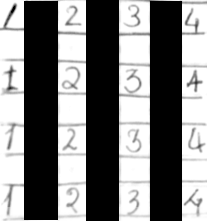
\includegraphics[scale=0.5]{figures/charrec.png}
    \caption{Example of Machine Learning: Character recognition}
    \label{fig:charrec}
  \end{center}
\end{figure}

The "example data" with its \emph{label} is collectively called as \emph{training set}, and it is used to teach machine learning how the character with given label looks like, so that ML can recognize when it encounters similar data in future. Machine learning can be applied in wide range of applications where it is not possible to express expertise but a large amount of sample data is available. Typical applications of machine learning include computer vision, pattern recognition, spam filtering, search result optimization etc. 

\section{Types of learning algorithms}
Based on application, ML algorithms can be can be classified in two major categories \emph{viz.} supervised learning and unsupervised learning. 

\emph{Supervised learning} algorithms are used when labels of the data to be are known. A spam filter is a good example where supervised learning can be used for \emph{classification}. Here we know an email received is either "spam" or "not-spam", these categories can be used as labels for the sample population and learning algorithm can classify within these two type.  One more application of supervised learning is to predict a numerical value in \emph{regression}. Consider a problem to predict value of a used property, the input parameters in this case are initial value, year of construction, size of property, locality and so on, whereas output is current resale value. one can construct a training set of known resale values and receptive values of input parameters and train leaning algorithm to predict other inputs. To generalize, aim in supervised learning is to learn mapping from input to output whose correct vales are provided by supervisor \cite{Alpaydin2004}.

\emph{Unsupervised learning} or \emph{clustering} is used in classification problems where the labels for the data are not known. An example of such problem is document clustering \cite{Alpaydin2004}. One of applications of document clustering is to cluster news reports which belong to same category like sport, science, art and so on. The number of such categories is not clear, and the machine learning application in such case needs to cluster articles based on some common words, and provide the supervisor data, which he may use to label clustered groups.

In case of fault classification, we have clearly defined taxonomy in earlier chapter, making our case as supervised classification problem. In following subsection, we define basic terms as applied to case of supervised learning.

\section{Basic concepts in machine learning}

A \emph{feature} $(x_i)$ is a result of measurement made on a unit input data. Generally, a set of features $(\boldsymbol{x}^t)$ is needed to characterize a unit of input data and is expressed as,
\[ \boldsymbol{x}^t = \left[ x_1, x_2, \ldots x_m \right]^T \]  
Its label $r$ denotes the class $C_i \in \{C_1, C_2 \ldots C_k\}$ it belongs to and is denoted as,
\[ r_i^t = \left\{ \begin{array}{ll}
         1 & \mbox{if $\boldsymbol{x}^t \in C_i$};\\
         0 & \mbox{if $\boldsymbol{x}^t \in C_j, j \neq i$}\end{array} \right. \] 
The training set $X$ is then defined as ordered set containing $N$ values of such examples,
\[ X = \{\boldsymbol{x}^t , \boldsymbol{r}^t \}_{t=1}^N  \]
The aim for machine learning algorithm is to learn values in training set and then classify new examples $\boldsymbol{x}$ by estimating value of $C(\boldsymbol{x})$. To achieve this, the algorithm tries to find out a hypotheses $h_i, i \in\{1,2, \ldots k\}$ from a set of all possible hypotheses such that,
\[ h_i(\boldsymbol{x}) = \left\{ \begin{array}{ll}
         1 & \mbox{if $\boldsymbol{x}^t \in C_i$};\\
         0 & \mbox{$\boldsymbol{x}^t \in C_j, j \neq i$}\end{array} \right. \] 
The \emph{empirical error} after training is calculated as,
\[ E(\{h\}_{i=1}^k|X) = \sum\limits_{t=1}^N \sum\limits_{i=1}^k | h_i(\boldsymbol{x}) \neq r_i^t ) | \]

Figure~\ref{fig:mlfitting} shows two possible hypotheses $h_1$ and $h_2$ for a simple 2-class classification problem, both with same value of empirical error and also actual boundary of classification $C$. If we choose hypothesis $h_1$ then the examples which lie in region between $h_1$ and $C$ will get incorrectly classified and this is called as \emph{overfitting}. On the other hand, if we choose $h_2$ then same will happen for examples in region between $C$ and $h_2$, called \emph{underfitting}. To avoid this and to get a hypothesis which is as close to $C$ as possible, typically one more labeled dataset with examples other than training set called as \emph{cross-validation set} is picked. The empirical error is then calculated over this set and hypotheses obtained during training and the hypothesis with least value of error is then selected. 

\begin{figure}[h]
  \begin{center}
    \captionsetup{justification=centering}
    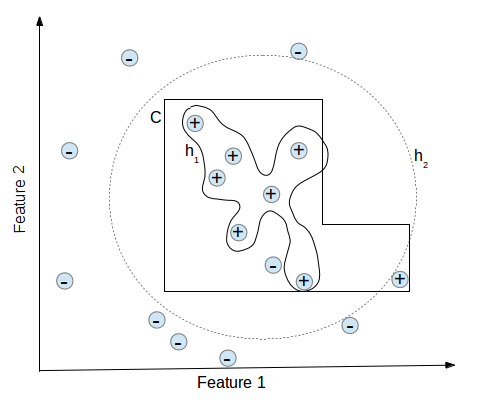
\includegraphics[scale=0.45]{figures/mlfitting.png}
    \caption{Example of overfitting and underfitting}
    \label{fig:mlfitting}
  \end{center}
\end{figure}

We use the term \emph{sample population} collectively for training set and cross-validation set.

\section{Machine Learning Algorithms for Classification}
\label{sec:c3mlclassification}
This section provides a brief overview of some of the most frequently used machine learning algorithms for classification problem. It includes advantages and disadvantages for individual algorithms.

\subsection{Na\"{i}ve Bayes}
Na\"{i}ve Bayes is a type of Bayesian classifier. It is one of most simple algorithms for learning, however in some cases it may outperform most sophisticated learning algorithms \cite{John1995}. Na\"{i}ve Bayes uses maximum-likelihood estimation to classify new examples. It is based on Bayesian theorem which states,
\[ posterior = \frac{likelihood \times prior}{evidance} \]
During training of Na\"{i}ve Bayes, probability of each class is calculated and stored as prior probability for that class. It also calculates probability for instances $\boldsymbol{x}$ given its class $c$. Under the assumption that attributes in $\boldsymbol{x}$ are independent, it simply becomes product of probabilities of each single attribute \cite{Williams2006}.
Hence Bayesian theorem, when applied to classification problem using Na\"{i}ve Bayes, becomes
\[ P(C_i|\boldsymbol{x}) = \frac{P(\boldsymbol{x}|C_i) \times P(C)}{P(\boldsymbol{x})}\]
A class $C_i$ is chosen if $P(C_i|x) = \max\limits_{k} \{ P(C_k|x)\}$.

A clear advantage of using Na\"{i}ve Bayes is that, it is fast to train and fast to classify data. This is because it needs to scan the database to compute probabilities and store it in a table during training and use this table to classify future examples. Also Na\"{i}ve Bayes is inherently not sensitive to irrelevant features as likelihood of class is product of probabilities of each single attribute. On the other hand for prior probabilities to be realistic, the sample population needs to be truly representative of actual data. Another major disadvantage is that the classifier assumes features to be independent of each other. However in many cases Na\"{i}ve Bayes classifier performs reasonably well even in cases where features are dependent on each other \cite{John1995, Williams2006}.

\subsection{Decision Trees}
\emph{Decision trees} are hierarchal models, wherein each step is a simple test against a threshold value or nominal attribute against set of all possible values \cite{Kotsiantis2013}. The steps are called as \emph{decision nodes} and test is implemented in form of a function on features $\boldsymbol{x}$ of example, with discrete outcomes represented as branches. These nodes apply tests recursively, as a example flows down the tree until it hits a \emph{leaf node}, which represents output (class in case of classification) \cite{Alpaydin2004}.

\begin{figure}[h]
  \begin{center}
    \captionsetup{justification=centering}
    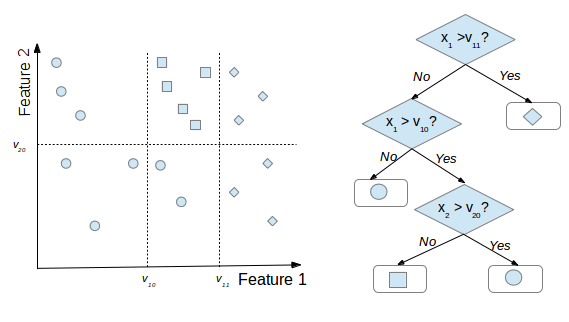
\includegraphics[scale=0.65]{figures/desctree.png}
    \caption{Example of decision tree}
    \label{fig:desctree}
  \end{center}
\end{figure}

In terms of a computer program, this algorithm devices a set of rules which can be interpreted as nested \texttt{IF-ELSE} structure. A simple decision tree is illustrated in figure~\ref{fig:mlfitting}. \emph{Decision tree learning} algorithms are used to obtain decision trees. ID3, RIPPER, C4.5 are some examples of these algorithms \cite{Mitchell1997}. ID3 \cite{Quinlan1986} is simplest of these algorithms. In case of decision trees, training is to choose a feature which provides the most information about training set. It then constructs tree using top-down approach. Other advanced algorithms like RIPPER \cite{Cohen1995} build upon same approach and then employ \emph{pruning} to reduce training error.

Decision tree use \enquote{white-box} approach, wherein the internal decision making and structure of tree is visible to user. This also make decision trees easy to visualize and interpret \cite{Kotsiantis2013}. Decision trees also perform feature screening to put less informative features near the leaf nodes, by its construction. Disadvantage of decision trees is that they can create over-complex trees that do not generalize the data well \emph{i.e.} overfitting of data. The problem of learning decision trees is known to be NP-complete hence its worst-case training speed can be slow \cite{Hyafil1976}.

\subsection{Multi-Layer Perceptrons}
\emph{Multi-Layer Perceptrons} (MLP) is a type of artificial neural network models and has been in use since the early 80's. In this model, each feature and outputs are represented as nodes, and feature nodes in each layer are connected to upper layer using weights or \emph{synapses}. Figure~\ref{fig:perceptron} is an example of a simple, single layered perceptron. The inputs $x_1, x_2 \ldots x_k$ are features and $x_0 = +1$ is a \emph{bias element}, used to make model more general by allowing user to fine-tune output by shifting output function.

\begin{figure}[h]
  \begin{center}
    \captionsetup{justification=centering}
    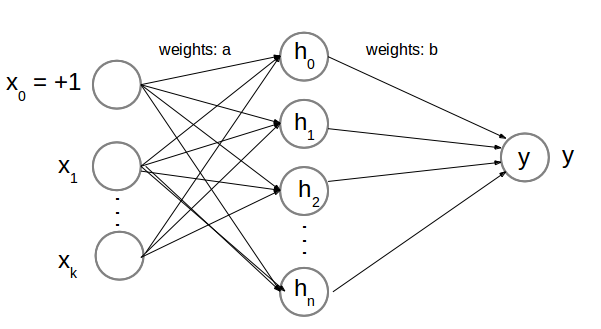
\includegraphics[scale=0.45]{figures/perceptron.png}
    \caption{Single layered perceptron}
    \label{fig:perceptron}
  \end{center}
\end{figure}

The output of perceptron in figure~\ref{fig:perceptron} can be represented mathematically as
\[ y = \sum\limits_{i=1}^k w_ix_i + w_0 \]
During training of perceptron, training algorithm will try to find appropriate connecting weights. Multiple layers of perceptrons can be constructed by implementing hidden layer of nodes between features and output, by doing so one can implement non-linear output functions. The degree of nonlinearity depends on number of hidden layers. Backpropagation algorithm \cite{Rumelhart1985} is one of commonly used algorithm for training MLPs. It works by calculating error correlations at each output and use these to calculate error terms in previous layers and so on. The error terms are then used to adjust weights of individual synapses.

Once trained, MLPs are able to classify data fast \cite{Alpaydin2004}. They can implement higher order polynomial functions and are flexible and powerful due to well researched mathematical background and variety of training algorithms available, which can be selected according to application and amount of data available. A disadvantage is that the network needs to be completely re-trained when new training data is to be added. Selection of features also has a profound impact on performance of MLPs \cite{Kavzoglu2002, El-Khatib2010}.

\subsection{Support Vector Machines}

\emph{Support Vector Machines} (SVMs) have existed for a long time, but the research on these gained particular momentum since Vapnik \cite{Vapnik1995} emphasized these methods in books on statistical learning theory. SVM belongs to class of linear classifiers.In higher dimensions, SVM tries to divide the feature space using decision hyperplanes. However as there can be several planes that divide feature space, SVM selects the plane with maximum margin. Figure~\ref{fig:svm1} shows a case where two possible lines divide feature space, $h_1$ and $h_2$. SVM will choose $h_2$ as \emph{decision boundary} or \emph{discriminant function} as it provides maximum margin for classification. The examples in training data SVM uses to evaluate maximum margin (\emph{i.e.} examples with least distance from decision hyperplane) are called \emph{support vectors}.

\begin{figure}[h]
  \begin{center}
    \captionsetup{justification=centering}
    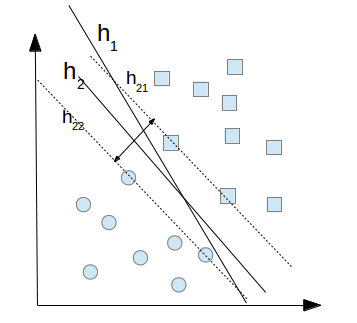
\includegraphics[scale=0.45]{figures/svm1.png}
    \caption{SVM with linear decision boundary}
    \label{fig:svm1}
  \end{center}
\end{figure}
The discriminant used in this case can be expressed as,
\[g(x) = \boldsymbol{w^T}\boldsymbol{x} + w_0 \]
Where $w_0$ denotes a bias, and vector $\boldsymbol{w}$ is known as weight factor.

However as illustrated in figure~\ref{fig:svm2} the feature space may not be linearly separable at all. In these cases SVM uses \emph{kernel trick} to achieve linearly separable kernel space. The idea behind kernel trick is to apply a function $\phi$ to transform all points in feature space, so that resulting feature space is linearly separable. After transformation, regular SVM algorithm is used for classification.

\begin{figure}[h]
  \begin{center}
    \captionsetup{justification=centering}
    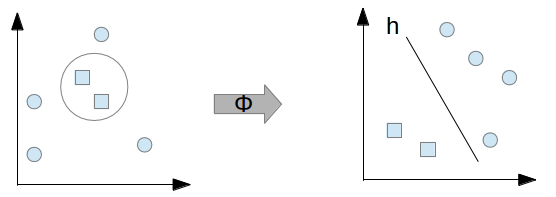
\includegraphics[scale=0.45]{figures/svm2.png}
    \caption{Kernel trick for SVM}
    \label{fig:svm2}
  \end{center}
\end{figure}

This makes the linear discriminant used of the form,
\[\boldsymbol{y} = \boldsymbol{w^T}\phi(\boldsymbol{x}) + w_0 \]

Referring to figure~\ref{fig:svm1}, hyperplane $h_2$ is actually a result of two hyperplanes, defined by the respective support vectors of two classes. Let $h_{21}$ and $h_{22}$ represent these hyperplanes	such that:
\[\begin{array}{ll} 
h_{21}: \boldsymbol{w^T}\boldsymbol{x} + b = 1 & \mbox{when label is +1};\\
h_{22}: \boldsymbol{w^T}\boldsymbol{x} + b = -1 & \mbox{when label is -1}
\end{array} \]

Let $||\boldsymbol{w}||$ denote the distance between these hyperplanes. Then the training of SVM is to find a maximum margin hyperplane, which can be viewed as an optimization problem \cite{Vapnik1995, Chang2011},
\[\begin{array}{ll} 
 \min &\frac{1}{2} ||\boldsymbol{w}||^2 \\
 \mbox{subject to} & r^t(\boldsymbol{w^T}\phi(\boldsymbol{x}) + w_0) 
\end{array}\]

The advantage of using SVM is its ability to tackle non-linear data. By using variey of kernels like linear, polynomial, RBF and so on, user has flexibility to classify data with non-linear feature spaces \cite {Chang2011}. Handling higher dimensional features spaces is also non-issue because of theoretical framework \cite{Vapnik1995} supports an $n$-dimensional space. SVMs also provide a unique solution as optimality problem is convex, which is an advantage as compared to neural networks, which can provide solutions at local minimum \cite{Auria2008}. SVM, being a maximum margin classifier, avoids underfitting of data. One the other hand, training an SVM is solving an optimality problem (known to be NP hard) and is quadratic (dependent of $N^2$), hence it can take a long time to train when datasets are large. Also, a common disadvantage of SVM is lack of transparency of the model it constructs to classify data, specially when feature set is large \cite{Auria2008}.
